\section{Test de la dichotomie}

\q{Tester votre fonction en donnant après reconnaissance graphique les 3
  solutions de l’équation $e^x=3x^2$ à $10^{-6}$ près.\\
  Vérifier que le produit des solutions vaut : }\il{-1.559156}\q{.}

\begin{dinglist}{111}
  \item Je trace la fonction :
  \codeFromFileT{main.py}{section-05/qa.py}
  \begin{center}
    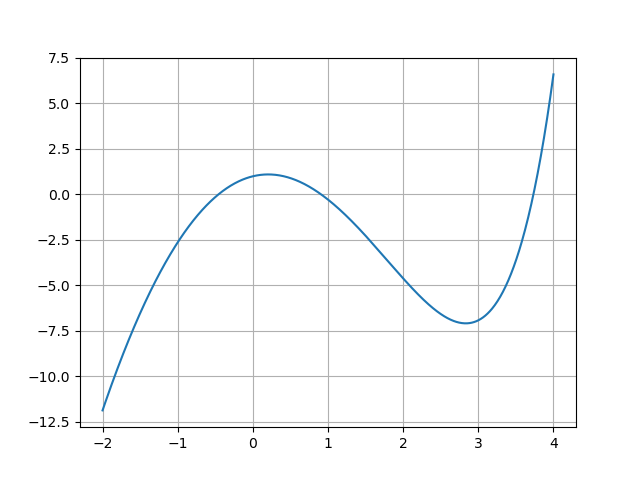
\includegraphics[scale=0.6]{section-05/qb.png}
  \end{center}
  \item J'en déduit les 3 intervalles :
  \[
    \left\{
    \begin{array}{c}
      \left[-1, 0\right] \\
      \left[0, 1\right]  \\
      \left[3, 4\right]  \\
    \end{array}
    \right.
  \]
  \item Je résous grâce à \il{dicho}:
  \codeFromFileT{main.py}{section-05/qc.py}
  Ce qui affiche \il{True}.
\end{dinglist}

